\chapter{Experiment Result}
\hspace*{6mm}For checking and validating the proposed method, we set up experiments from technical and clinical perspective. In technical perspective, admittance control, force-guided alignment, and file feedrate control were conducted and verified. On the other hand, The acrylic root model before and after the experiment were also compared in this chapter. 
\section{Experimental Setup}
\hspace*{6mm}To control all devices with low latency, a communication protocol - EtherCAT and a real-time oprating system (RTOS) are interfaced. Every devices are connected in Daisy-chain shown in Fig \ref{fig:EtherCAT}. EtherCAT (Ethernet for Control Automation Technology) is constructed on EtherNET and uses "processing on the fly" technology to provide short cycle time (less than 100 $\mu$s) and low jitter \cite{web5}.
\begin{figure}[htbp]
\begin{center}
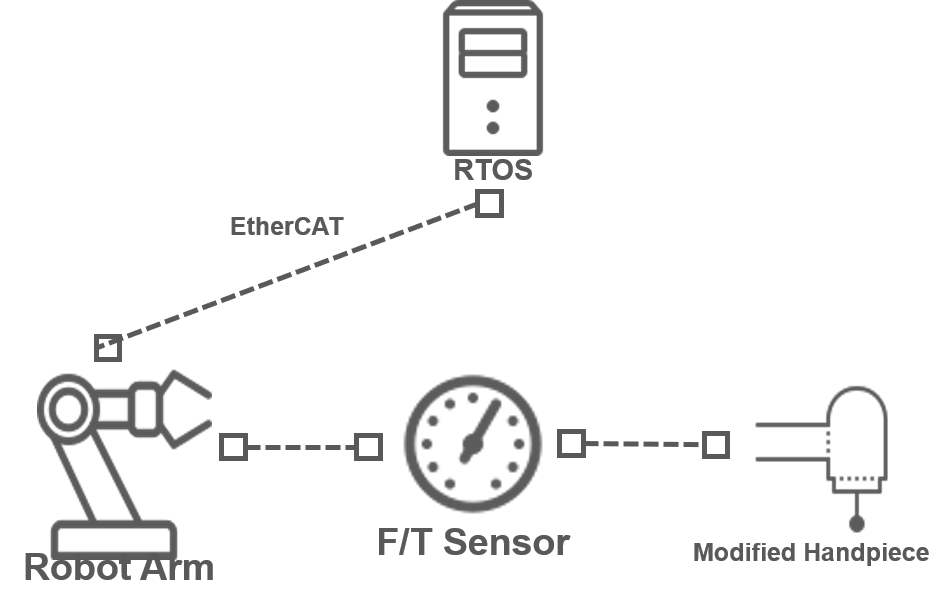
\includegraphics[width=0.7\linewidth]{Images/EtherCAT.png}
\caption{System integration and communication protocol.}
\label{fig:EtherCAT}
\end{center}
\end{figure}

\begin{figure}[htbp]
\begin{center}
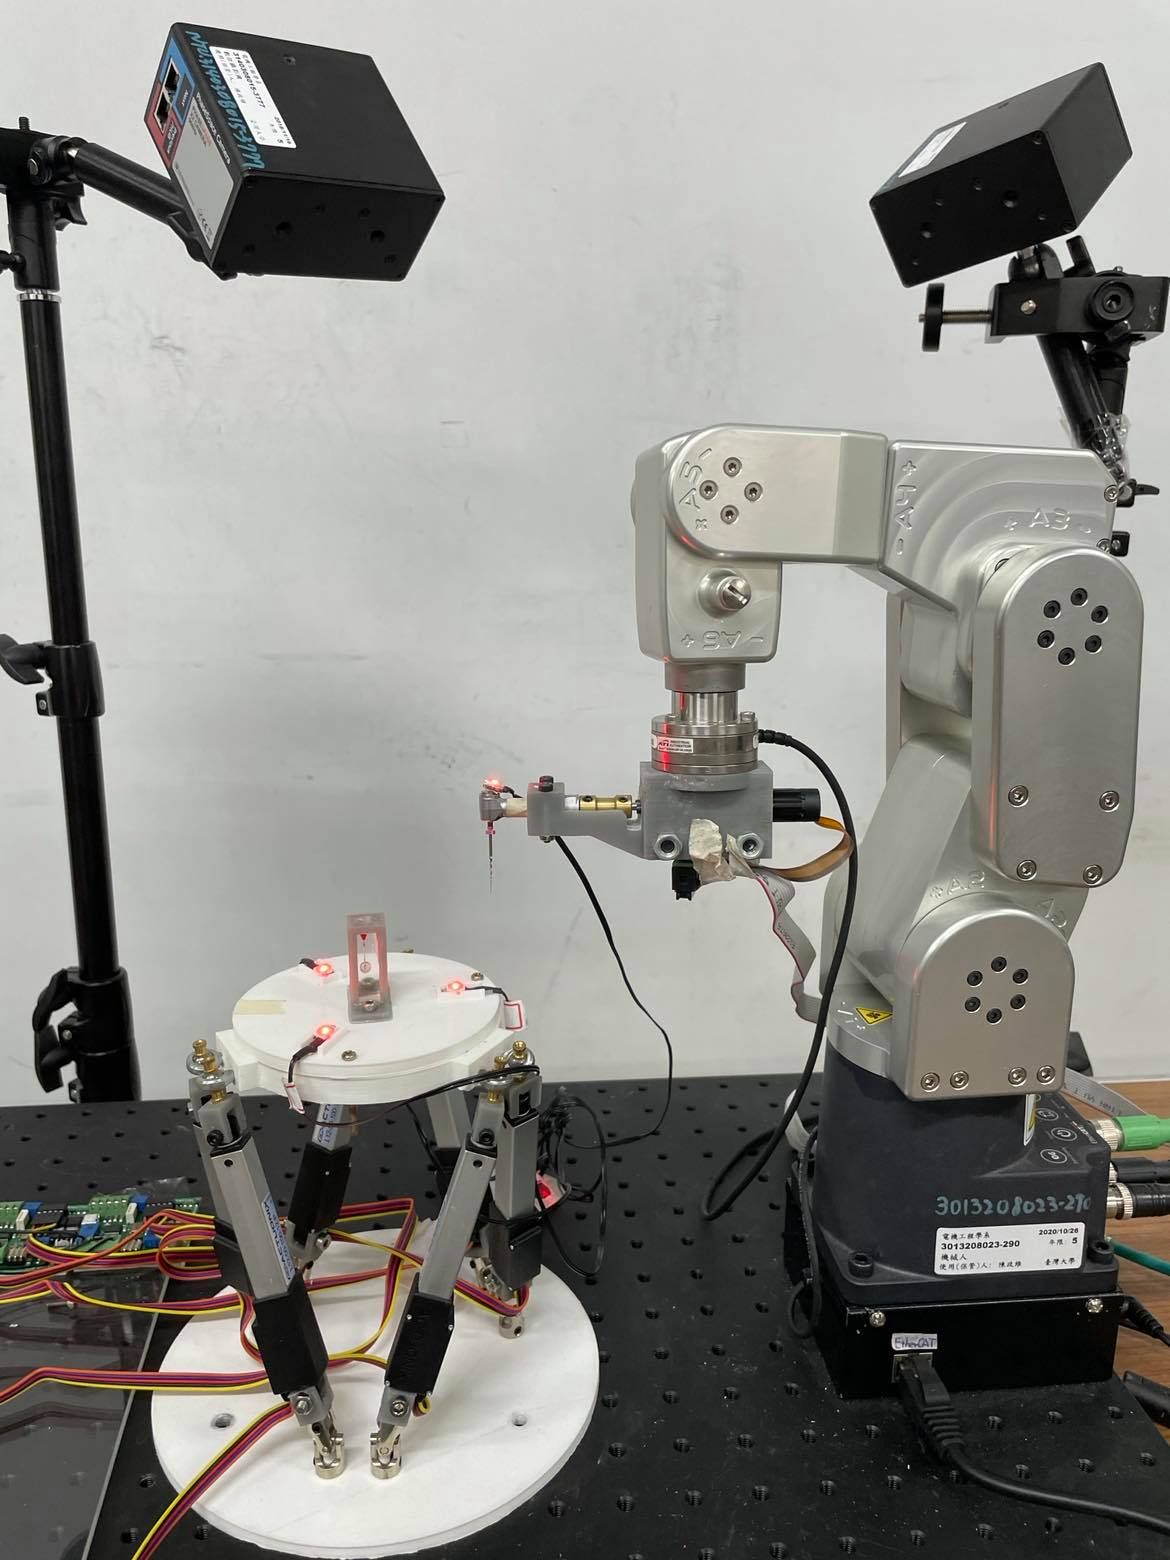
\includegraphics[width=0.6\linewidth]{Images/System.jpg}
\caption{Experimental setup.}
\label{fig:system}
\end{center}
\end{figure}
\par
Moreover, for the position information and simulating patient moving, A motion capture system and a Stewart Platform were set up shown as Fig \ref{fig:system}. All of the specifications of the hardware and software environments are listed in Table \ref{tab:exp_specification}.

\begin{table}[htbp]
\centering
\caption{Specifications of the hardware and software environments}
\label{tab:exp_specification}
\par
\begin{tabular}{c|c} 
\hline \hline
Item											&Specification					\\	\hline
Development Environment							&LabVIEW 2018					\\	\hline
\multirow{2}{*}{Real-Time Operating System}		&National Instrument-RT target	\\
												&CPU: Intel Core 8				\\	\hline
Communication Protocol							&EtherCAT						\\	\hline
Robot Arm										&Mecademic-Meca500				\\	\hline
F/T Sensor										&ATI-Mini40						\\	\hline
\multirow{2}{*}{Motor}							&Maxon 24V DC motor				\\
												&Gear ratio: 67					\\	\hline
\multirow{2}{*}{Motion Capture System}			&PhaseSpace-Impulse X2E 		\\
												&Resolution: 1mm				\\	\hline
Steward Platform								&Linear Actuator: 				\\	
\hline \hline
\end{tabular}
\end{table}

\begin{figure}[htbp]
\begin{center}
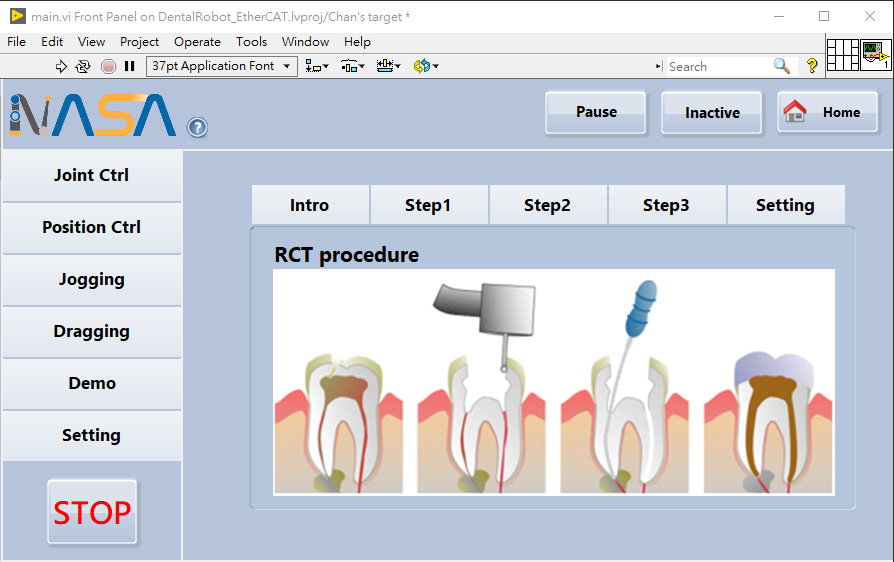
\includegraphics[width=1\linewidth]{Images/GUI.png}
\caption{Graph user interface with LabVIEW 2018}
\label{fig:GUI}
\end{center}
\end{figure}
\section{Admittance Control}
\hspace*{6mm}In order to prove the validation of admittance control, we set up this experiment. Here we build a Stewart platform, which has six degrees of freedom and provide a slight movement. We use a Stewart platform to simulate a motion of a patient. Basically, when the patient moves to a position, our system should move to the same place. Therefore, we plan to observe the target's and the handpiece's position to validate that our system can track the patient. Besides, we use PhaseSpace to obtain their motion in real-time. PhaseSpace is a motion capture device whose resolution is around $1$ mm. Before starting this experiment, we should fix a relative position between the file and the acrylic tooth. We made the file rotate and get stuck in the root canal of an acrylic model. Then we used "Doctor dragging" mode to install the acrylic model on the Stewart platform. Therefore, we can guarantee that the relative position between the file and the acrylic tooth.
\par
We moved the Stewart platform in horizontal and vertical directions separately. The motion planning in the horizontal direction is a square which is $10\times 10$ mm and in the vertical direction is a linear motion from $0$ to $40$ mm.
\section{Automatically Direction Changing}
Validation of Self-alignment Mode
\par\noindent
(Metrics: time, completeness and file breakage)								
\par\noindent
(Completeness definition: comparison of pixel area before and after experiment via image)
\section{Repetitive Experiment}
validation of repetitive experiment
\par\noindent
(Metrics: file breakage, compare with and without reverse)